%%%%%%%%%%%%%%%%%%%%%%%%%%%%%%%%%%%%%%%%%
% Plasmati Graduate CV
% LaTeX Template
% Version 1.0 (24/3/13)
%
% License:
% CC BY-NC-SA 3.0 (http://creativecommons.org/licenses/by-nc-sa/3.0/)
%
% Important note:
% This template needs to be compiled with XeLaTeX.
% The main document font is called Fontin and can be downloaded for free
% from here: http://www.exljbris.com/fontin.html
%
%%%%%%%%%%%%%%%%%%%%%%%%%%%%%%%%%%%%%%%%%

%----------------------------------------------------------------------------------------
%	PACKAGES AND OTHER DOCUMENT CONFIGURATIONS
%----------------------------------------------------------------------------------------

\documentclass[a4paper,10pt]{article} % Default font size and paper size

\usepackage{fontspec} % For loading fonts
\defaultfontfeatures{Mapping=tex-text}
\setmainfont[SmallCapsFont = Fontin SmallCaps]{Fontin} % Main document font

\usepackage{xunicode,xltxtra,url,parskip} % Formatting packages

\usepackage[usenames,dvipsnames]{xcolor} % Required for specifying custom colors

\usepackage{savetrees}
\usepackage{longtable}

\usepackage[big]{layaureo} % Margin formatting of the A4 page, an alternative to layaureo can be \usepackage{fullpage}
% To reduce the height of the top margin uncomment: \addtolength{\voffset}{-1.3cm}

\usepackage{hyperref} % Required for adding links	and customizing them
\definecolor{linkcolour}{rgb}{0,0.2,0.6} % Link color
\hypersetup{colorlinks,breaklinks,urlcolor=linkcolour,linkcolor=linkcolour} % Set link colors throughout the document

%\usepackage{picins}
\usepackage{titlesec} % Used to customize the \section command
\usepackage{savetrees}
\titleformat{\section}{\Large\scshape\raggedright}{}{0em}{}[\titlerule] % Text formatting of sections
\titlespacing{\section}{0pt}{5pt}{4pt} % Spacing around sections

\begin{document}

\pagestyle{empty} % Removes page numbering
%\parpic[r]{\includegraphics[width=0.27\textwidth]{bewerbungsbild-1.jpg}}
\font\fb=''[cmr10]'' % Change the font of the \LaTeX command under the skills section

%----------------------------------------------------------------------------------------
%	NAME AND CONTACT INFORMATION
%----------------------------------------------------------------------------------------

\par{\centering{\Huge Vaibhav \textsc{Kasturia}}\bigskip\par} % Your name

\section{Personal Data}

\begin{minipage}[b][4.5cm][t]{0.5\textwidth}
\begin{tabular}{ll}
\textsc{Place of Birth:} & Delhi, India \\ 
\textsc{Date of Birth:} & 18 November 1992 \\
\textsc{Nationality:} & Indian (Permanent Resident of Germany)\\
\textsc{Address:} & Schwannstr. 6, 40476 Düsseldorf, Germany \\
%\textsc{Phone:} &  +49 ---------\\
\textsc{Email:} & \href{mailto:vkasturia@deloitte.de}{vkasturia@deloitte.de}, \href{mailto:vbh18kas@gmail.com}{vbh18kas@gmail.com} \\
\textsc{LinkedIn:} & \href{https://www.linkedin.com/in/vkasturia/}{vkasturia} \\
\textsc{Github:} & \href{https://github.com/vkasturia}{vkasturia} \\
\textsc{Webpage:} & \href{https://www.vaibhavkasturia.com}{www.vaibhavkasturia.com}
\end{tabular}
\end{minipage}
\begin{minipage}[b][4.5cm][t]{0.5\textwidth}
\hspace{3.5cm}
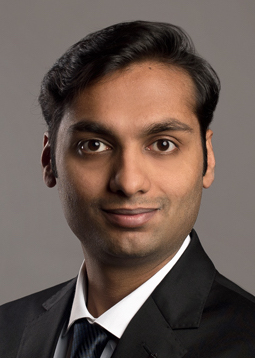
\includegraphics[width=0.3\textwidth]{./bewerbungsbild_cropped.jpg}
\end{minipage}
\\[-3.5em]

%----------------------------------------------------------------------------------------
%	EDUCATION
%----------------------------------------------------------------------------------------

\section{Education}

\begin{tabular}{l p{0.8\linewidth}}	
\textsc{2015 - 18} & \mbox{Master of Science in \textsc{Internet Technologies and Information Systems (ITIS)}}\\
& \textbf{Leibniz University Hannover}, Hannover\\
& Major: Data and Information\\
& Research Project: ``Building \& Querying Semantic Layers for Web Archives''\\
& Thesis: \mbox{``Ranking Archived Documents for Structured Queries on Semantic Layers''} 
\\
&\normalsize \textsc{GPA}: 1.1 (German Scale)\\
&\\

%------------------------------------------------

\textsc{2011 - 15} & Bachelor of Engineering (Hons.) in \textsc{Computer Science}\\
& \textbf{Birla Institute of Technology and Science - Pilani}, Dubai\\
& Thesis: \mbox{``Software Development Practices at ESRI''}\\
&\normalsize \textsc{GPA}: 1.1 (German Scale), 9.77 (Indian Scale)\\
&\\

\end{tabular}


%----------------------------------------------------------------------------------------
%	WORK EXPERIENCE 
%----------------------------------------------------------------------------------------

\section{Work Experience}

\begin{longtable}{l p{11cm}}
\textsc{May 2021 - Present} & Consultant at \textsc{Deloitte}, Düsseldorf\\
& \emph{\href{https://www2.deloitte.com/de/de/pages/risk/solutions/digital-ai-controls-and-algorithms.html}{Digital / AI Controls / Algorithms}, \href{https://www2.deloitte.com/de/de/services/risk.html?icid=bottom_risk}{Risk Advisory}}\\[1mm]
& \textbf{\footnotesize{ML Text Extraction of Securities Prospectuses}}\vspace{0.2em}
  {\footnotesize
  	\begin{itemize}
  		\setlength\itemsep{0.2em}
 		\item Built a prototype that uses AI and rule-based solutions to recognize, extract, and display relevant data from the documents.      
  \end{itemize}
  }
\\[-4mm]
& \textbf{\footnotesize{Explainable AI}}\vspace{0.2em}
  {\footnotesize
  	\begin{itemize}
  		\setlength\itemsep{0.2em}
 		\item Developed a tool which uses Shapley values to explain the decision-making process of Deep Learning models like BERT, RoBERTa and DistilBERT.      
  \end{itemize}
  }
\\
\multicolumn{2}{c}{} \\[-1.5em]

%------------------------------------------------

\textsc{Aug 2018 - Oct 2020} & Research Associate at \textsc{University of Halle-Wittenberg}, Halle (Saale)
\\
& \emph{Big Data Analytics, \href{https://webis.de}{Webis Group}}\\[1mm]
& \textbf{\footnotesize{Query Understanding via Entity Linking}}\vspace{0.2em}
  {\footnotesize
  	\begin{itemize}
  		\setlength\itemsep{0.2em}
 		\item \textbf{Goal:} Interpret ambiguous search engine queries to show more relevant results to the user, answer the query or help fill search engine's knowledge boxes. 
 		\item Designed and developed an automatic approach that uses query segmentation and entity linking to identify the most reasonable interpretations of a query based on the contained entities. 
		\item Conducted an experimental comparison on a new corpus of 2,800~queries. It proves that my approach has better interpretation accuracy at a better run time than the previously best methods.    
  \end{itemize}
  }
\\[-2mm]
& \textbf{\footnotesize{Total Recall in Systematic Reviews}}\vspace{0.2em}
  {\footnotesize
  	\begin{itemize}
  		\setlength\itemsep{0.2em}
 		\item \textbf{Goal:} Find all relevant documents (“total recall”) given a collection of potentially several thousands of documents somewhat related to a user-specified topic. A single systematic review may take up to 2 years without any machine-assistance. 
 		\item Built a system that reduces the review period by ordering these documents in descending relevance. 
 		\item Implemented several machine learning methods from an existing total recall approach (\href{https://github.com/hical/HiCAL}{HiCAL}) and tested these on botanical research datasets. The results show that machine learning reduces the human effort by almost 80 percent. 
		\item Development of a new algorithm that continuously adapts the feature set to the growing user feedback, and combines the current feature set with machine learning (learning-to-rank) to a ranking score.    
  \end{itemize}
  }
\\[-2mm]
& \textbf{\footnotesize{Argumentative Axiomatic Re-Ranking for Medical Search Queries}}\vspace{0.2em}
  {\footnotesize
  	\begin{itemize}
  		\setlength\itemsep{0.2em}
 		\item People use search engines to seek health advice online. 
		\item Using search engines to complete such decision making tasks, users are not able to discern authoritative from unreliable information.
		\item As part of a team, we developed an axiomatic approach to re-rank search results obtained by traditional search models, in order to promote more argumentative results for medical queries.   
  \end{itemize}
  }
\\[-2mm]
& \textbf{\footnotesize{Activities}}\vspace{0.2em}
  {\footnotesize
  	\begin{itemize}
  		\setlength\itemsep{0.2em}
 		\item Prepared and took exercises for undergraduate and graduate courses (Object Oriented Programming in Java, C Programming, Search Algorithms, Foundations of Computer Science and Concepts of Modelling).
 		\item Supervised a team of 10 students in their software project internship. \newline \textbf{Topic:} Develop a system to automatically migrate a company's old Excel-records in Excel to a database.
 		\item Maintenance of the \href{https://www.informatik.uni-halle.de/arbeitsgruppen/big_data_analytics/}{Big Data Analytics} webpage.    
  \end{itemize}
  }
\\
\multicolumn{2}{c}{} \\[-1.5em]
%------------------------------------------------

\textsc{May 2018 - Jul 2018} & Research Associate at \textsc{Fraunhofer IAIS}, Bonn\\[-1em]
& {\footnotesize
  	\begin{itemize}
  		\setlength\itemsep{0.2em}
 		\item Prototyped a Question Answering system for an accounting firm.
		\item As part of the team, contributed to the development of algorithms in the area of Deep Learning as well as Speech Processing for intelligent smart car systems.
		\item Small contributions to the project GEISER which dealt with the analysis of spatial data. 
  \end{itemize}
  }\\
\multicolumn{2}{c}{} \\[-1.5em]

%------------------------------------------------

\textsc{Oct 2016 - Jan 2018} & Student Assistant at \textsc{L3S Research Center}, Hannover\\[1mm]
& \textbf{\footnotesize{\href{http://alexandria-project.eu/}{ALEXANDRIA Project}}}\vspace{0.2em}
  {\footnotesize
  	\begin{itemize}
  		\setlength\itemsep{0.2em}
 		\item Research on methods for the semantic and entity-based exploration of Web Archives. 
 		\item Aim of the project was to significantly advance semantic and time-based indexing for Web Archives, to efficiently index, retrieve and explore information about entities and events from the past.
		\item Built semantic profiles (“layers”) that describe semantic information about the
		contents of Web Archives using Entity Linking Tools.
		\item Evaluated the semantic layers for complex information needs against keyword-based search
systems like Google, Bing and HistDiv.
		\item Designed and evaluated statistical and advanced models (PageRank-like) to
		rank results returned by running queries on these layers.    
  \end{itemize}
  }\\
 \multicolumn{2}{c}{} \\[-1.5em]

%------------------------------------------------

\textsc{Aug 2014 - Jan 2015} & Software Developer (Intern) at \textsc{ESRI}, Sharjah\\[-1em]
& {\footnotesize
  	\begin{itemize}
  		\setlength\itemsep{0.2em}
 		\item Handled Multidimensional Geo-data (GRIB, NetCDF, HDF, etc.)
		\item Analyzed Raster, Mosaic and Image Service Data Layers.
 		\item Fixed bugs and changes requested for ArcGIS 10.
		\item Validated UI functioning of Raster and Geo-Processing Tools of ArcGIS Pro.
		\item Removed potential defects (by Coverity Analysis) in Raster Solutions of ArcGIS 10.    
  \end{itemize}
  }\\
\multicolumn{2}{c}{} \\

\end{longtable} 
\vspace{-3em}

%----------------------------------------------------------------------------------------
%	TECHNICAL PROFICIENCY 
%----------------------------------------------------------------------------------------

\section{Technical Proficiency}

\begin{tabular}{ll}
\textbf{Programming Languages:} & \textsc{Java}, Python, \textsc{C/C++}\\
\textbf{Data Science / Machine Learning:} & Shap, Transformers, NumPy, pandas, scikit-learn, Matplotlib\\
\textbf{Information Retrieval:} & Apache Lucene\\
\textbf{Database Systems:} & Graph database (Virtuoso), NoSQL database (RocksDB),\\ 
& SQL databases (My\textsc{SQL}, Postgre\textsc{SQL})\\
\textbf{Natural Language Processing:} & Entity Recognition, Entity Linking, Entity Disambiguation,\\
									  & Word Embeddings, Query Segmentation\\
\textbf{Java Frameworks/Libraries:} & Apache Maven, Apache Jena, Apache Tika, SparkJava,\\
							& Standard Libraries (Apache Commons, Apache Lang, etc.)\\
\textbf{Semantic Web Technologies:} & RDF/RDFa, \textsc{OWL}, \textsc{SPARQL}, Turtle\\
\textbf{Web Technologies:} & HTML5, CSS, Materialize/Bootstrap, Flask\\
\textbf{Geo-Information Systems:} & ArcGIS\\
\textbf{IDE Software:} & Jupyter Notebook, IntelliJ, Eclipse, NetBeans, Visual Studio\\
\textbf{Document Preparation:} & MS Office, Apple Office Suite, LaTeX\\
\textbf{Version-Control Software:} & Gitlab/Github, GitKraken, \textsc{SVN}, \textsc{CVS}\\
\textbf{Others:} & Docker, Multithreaded Programming\\
\textbf{Basic Knowledge:} & Intel 8085 Programming, Wireshark, Scilab\\
\end{tabular}
\\
\vspace{-0.5em}

%----------------------------------------------------------------------------------------
%	ACHIEVEMENTS AND AWARDS
%----------------------------------------------------------------------------------------

\section{Achievements and Awards}

\begin{tabular}{ll}
\textsc{Dec} 2018 & Best Master's degree certificate for 2017/18 by Leibniz University Hannover\\
\textsc{Jun} 2017 & Best Research Paper Award Nomination at at JCDL 2017\\
\textsc{2011 - 15} & BITS Scholarship for Academic Excellence for the entire Bachelor’s Degree\\
\end{tabular}

%----------------------------------------------------------------------------------------
%	PUBLICATIONS
%----------------------------------------------------------------------------------------

\section{Publications}

\begin{tabular}{ll}
\textsc{May 2021} & \href{https://arxiv.org/pdf/2105.08581.pdf}{\textsc{Entity-Based Query Interpretation}}\\
& \textbf{Vaibhav Kasturia}, Marcel Gohsen and Matthias Hagen \\
\end{tabular}

\begin{tabular}{ll}
\textsc{Nov 2019} & \href{https://webis.de/downloads/publications/papers/bondarenko_2019.pdf}{\textsc{Webis at TREC 2019: Decision Track}}\\
& A. Bondarenko, M. Fröbe, \textbf{V. Kasturia}, M. Völske, B. Stein and M. Hagen \\
& 28th International Text Retrieval Conference (TREC'19), Gaithersburg (Maryland, USA)\\
\end{tabular}

\begin{tabular}{ll}
\textsc{Jun 2018} & \href{https://dl.acm.org/doi/10.1145/3197026.3197049}{\textsc{Ranking Archived Documents for Structured Queries on Semantic Layers}}\\
& Pavlos Fafalios, \textbf{Vaibhav Kasturia} and Wolfgang Nejdl\\
& ACM/IEEE-CS Joint Conference on Digital Libraries (JCDL’18), Fort Worth (Texas, USA)\\
\end{tabular}

\begin{tabular}{ll}
\textsc{Nov 2017} & \href{https://arxiv.org/abs/1810.10455}{\textsc{Building and Querying Semantic Layers for Web Archives (Extended Version)}}\\
& Pavlos Fafalios, Helge Holzmann, \textbf{Vaibhav Kasturia} and Wolfgang Nejdl\\
& International Journal on Digital Libraries (IJDL)\\
\end{tabular}

\begin{tabular}{ll}

\textsc{Jun 2017} & \href{http://ieeexplore.ieee.org/document/7991555/}{\textsc{Building and Querying Semantic Layers for Web Archives}}\\
& Pavlos Fafalios, Helge Holzmann, \textbf{Vaibhav Kasturia} and Wolfgang Nejdl\\
& ACM/IEEE-CS Joint Conference on Digital Libraries (JCDL’17), Toronto (Ontario, Canada)\\
\end{tabular}

\begin{tabular}{ll}
\textsc{Jun 2017} & \href{http://ieeexplore.ieee.org/document/7991617/}{\textsc{Towards a Ranking Model for Semantic Layers over 
Digital Archives}}\\
& Pavlos Fafalios, \textbf{Vaibhav Kasturia} and Wolfgang Nejdl\\
& ACM/IEEE-CS Joint Conference on Digital Libraries (JCDL’17), Toronto (Ontario, Canada)\\
\end{tabular}
\\
%----------------------------------------------------------------------------------------
%	TECHNICAL CERTIFICATIONS
%----------------------------------------------------------------------------------------

\section{Technical Certifications}

\begin{tabular}{ll}
\textsc{Jun 2021} & \href{https://vaibhavkasturia.com/certificate/bsi-it-grundschutz-praktiker-vaibhav-kasturia.pdf}{\textsc{BSI IT-Grundschutz-Praktiker (Bitkom Akademie)}}\\
\textsc{Dec 2020} & \href{https://www.coursera.org/account/accomplishments/verify/ZF4WLZWMJR3U}{\textsc{Machine Learning, Stanford University (Coursera)}}\\
%\textsc{Oct 2020} & \href{https://www.udemy.com/certificate/UC-1c189099-d482-413f-8687-d15c337191b9/}{\textsc{Docker and Kubernetes: The Complete Guide (Udemy)}}\\
\textsc{Apr 2020} & \href{https://ninjasfiles.s3.amazonaws.com/certificate643308086b235198c8d9aa73fa674fe417597e.pdf}{\textsc{Competitive Programming (Coding Ninjas)}}\\
\textsc{Mar 2020} & \href{https://vaibhavkasturia.com/certificate/introduction-to-the-bash-shell-on-macos-and-linux-vaibhav-kasturia.pdf}{\textsc{Introduction to the Bash Shell on Mac OS and Linux (Pluralsight)}}\\
\textsc{Oct 2019} & \href{https://www.udemy.com/certificate/UC-1EV6KK7F/}{\textsc{Master Object Oriented Design in Java (Udemy)}}\\
\textsc{Sep 2019} & \href{https://www.udemy.com/certificate/UC-P7AJYXY6/}{\textsc{Complete Python Bootcamp (Udemy)}}\\
\textsc{May 2019} & \href{https://www.coursera.org/account/accomplishments/verify/XN25BG7WGAM3}{\textsc{Improving Deep Neural Networks (Coursera)}}\\
\textsc{May 2019} & \href{https://www.coursera.org/account/accomplishments/certificate/LWCFY27WJB9R}{\textsc{Structuring Machine Learning Projects (Coursera)}}\\
\textsc{May 2019} & \href{https://www.coursera.org/account/accomplishments/verify/KCVQACF5SKEM}{\textsc{Neural Networks and Deep Learning (Coursera)}}\\
\end{tabular}
\\
%----------------------------------------------------------------------------------------
%	EXTRA-CURRICULAR ACTIVITIES
%----------------------------------------------------------------------------------------

\section{Extra-Curricular Activities}

\begin{tabular}{ll}
\textsc{Oct 2019} & \textsc{Sub-Reviewer}\\
& ECIR 2020 Conference, Lisbon and CHIIR 2020 Conference, Vancouver\\
\\
\textsc{Sep 2016} & \textsc{Student Volunteer, Organizing Committee}\\
& TPDL 2016 Conference, Hannover\\
\\
\textsc{May 2016} & \textsc{Student Volunteer, Organizing Committee}\\
& ACM WebSci'16 Conference, Hannover\\
\\
\textsc{Sep 2012 - Jun 2013} & \textsc{General Secretary, Student Council}\\
& BITS Pilani, Dubai\\
\end{tabular}
\\
%----------------------------------------------------------------------------------------
%	LANGUAGES
%----------------------------------------------------------------------------------------

\section{Languages}

\begin{tabular}{lll}
\textsc{English:} & Native (C2) & IELTS General (\textsc{Oct 2019, Overall Band: 8.0/9.0})\\

\textsc{German:} & Advanced (C1) & Goethe-Certificate C1 ( \textsc{Jul 2020, Overall Score: 74/100})\\

\textsc{Hindi:} & Mother tongue &\\
\end{tabular}
\\
%----------------------------------------------------------------------------------------
%	INTERESTS AND ACTIVITIES
%----------------------------------------------------------------------------------------

\section{Interests and Activities}

Sketching, Swimming, Photography, Traveling
%----------------------------------------------------------------------------------------


\end{document}